\chapter{Trade-Off}
\label{ch:trad_off}
\setlength{\parindent}{15pt}

With the concepts chosen it is time to perform a trade-off to see which concept has the greatest potential to meet the expectations of the stakeholders. This assessment is critical to the project since it is not possible to enter the preliminary design phase with all of the concepts due to time and resource limitations. Therefore, it is crucial that the analysis is complete and unbiased. To achieve this, trade criteria are selected such that it is possible to judge the degree of compliance of all concepts to requirements most important to the stakeholders. The selection of the criteria and their influences on the final concept selection (weighting) are based on requirements that highly influence the design of the UAV, or that are most important to the key stakeholders. The score of each concept (determined by the criteria and their weights) ultimately indicates the most promising design.  

In \autoref{sec:comp_summ} the complete trade-off table is shown first, summarising the results of the sub-trade-offs described later in the report. \autoref{sec:comp_trad_crit} presents the reasoning for the selection of the trade criteria, and \autoref{sec:comp_crit_weig} shows the method of determining the weights of the trade criteria. Finally, the sensitivity analysis of the trade-off method is performed in \autoref{sec:sens_anal}.

\section{Summary}
\label{sec:comp_summ}

%colour codes
%red #FF0000            |   \cellcolor[HTML]{FF0000}
%orange #FF8000         |   \cellcolor[HTML]{FFC000}
%yellow #FFFF00         |   \cellcolor[HTML]{FFFF00}
%light green #00FF00    |   \cellcolor[HTML]{92D050}
%dark green #088A08     |   \cellcolor[HTML]{00B050}
%light blue #0000FF     |   \cellcolor[HTML]{0000FF}
%dark blue #08088A      |   \cellcolor[HTML]{08088A}

This section will present the results of the final trade-off, which can be seen in \autoref{tab:finaltradeoff}. The outcomes of the trade-off will briefly be discussed to get a grasp as to why the concepts scored as they did. Detailed explanation of the separate criteria scores are the result of extensive research on each criterion, the reasoning behind these scores can be found in \Cref{sec:perf_analy,sec:manostab,sec:grouhand,ch:costanal,ch:deverisk,ch:relianal}. For clarity, the table contains colours to give an overview of the severity of the scores. Five colours have been used in a 30-15-10-15-30 spacing (Red, Orange, Yellow, Light Green, Dark Green). This spacing has been used to show more detail around the average than around the extremes. For when there is a lack of colour, each score has a superscript showing which category it scores: 1 = Red, 2 = Orange, 3 = Yellow, 4 = Light Green, 5 = Dark Green. 

\begin{table}[H]
    \setlength\extrarowheight{5pt}
    \setlength\arrayrulewidth{1pt}
    \centering
    \caption{Final Trade-Off}
    \label{tab:finaltradeoff}
    \begin{tabular}{r|>{\centering}p{2.1cm}|>{\centering}p{1.9cm}|>{\centering}p{1.3cm}|>{\centering}p{1.1cm}|>{\centering}p{0.8cm}|>{\centering}p{0.7cm}|>{\centering}p{0.4cm}|c} 
    \textbf{Concept \rotatebox{90}{\hspace{0.5cm}Criterion}}        & 
    \rotatebox{90}{\textbf{Performance}}                            &
    \rotatebox{90}{\textbf{M\&S}}                                   & 
    \rotatebox{90}{\textbf{Reliability}}                            & 
    \rotatebox{90}{\textbf{Production Cost}}                        & 
    \rotatebox{90}{\textbf{Development Risk}}                       &
    \rotatebox{90}{\textbf{Sustainability}}                         &
    \rotatebox{90}{\textbf{Ground Handling}}                        &
    \rotatebox{90}{\textbf{Outcome}}
    \\\hline
    Tailsitter      &
    \cellcolor[HTML]{FFFF00}50$^{^3}$ &
    \cellcolor[HTML]{FFFF00}46$^{^3}$ &
    \cellcolor[HTML]{FFFF00}50$^{^3}$ &
    \cellcolor[HTML]{FFFF00}50$^{^3}$ &
    \cellcolor[HTML]{00B050}75$^{^5}$ &
    \cellcolor[HTML]{00B050}84$^{^5}$ &
    \cellcolor[HTML]{92D050}59$^{^4}$ &
    \cellcolor[HTML]{FFFF00}\textbf{55$^{^3}$}
    \\[5pt]\cline{2-8}\cdashline{1-1}\cdashline{9-9}
    Tandem          &
    \cellcolor[HTML]{FF0000}17$^{^1}$ &
    \cellcolor[HTML]{FFC000}41$^{^2}$ &
    \cellcolor[HTML]{FFC000}43$^{^2}$ &
    \cellcolor[HTML]{FFC000}35$^{^2}$ &
    \cellcolor[HTML]{FFC000}35$^{^2}$ &
    \cellcolor[HTML]{FF0000}25$^{^1}$ &
    \cellcolor[HTML]{FFC000}38$^{^2}$ &
    \cellcolor[HTML]{FFC000}\textbf{33$^{^2}$}
    \\[5pt]\cline{2-8}\cdashline{1-1}\cdashline{9-9}
    Prandtl Box     &
    \cellcolor[HTML]{92D050}67$^{^4}$ &
    \cellcolor[HTML]{FFC000}41$^{^2}$ &
    \cellcolor[HTML]{92D050}68$^{^4}$ &
    \cellcolor[HTML]{FFFF00}50$^{^3}$ &
    \cellcolor[HTML]{92D050}70$^{^4}$ &
    \cellcolor[HTML]{92D050}58$^{^4}$ &
    \cellcolor[HTML]{FFFFFF}54$^{^3}$ &
    \cellcolor[HTML]{92D050}\textbf{58$^{^4}$}
    \\[5pt]\cline{2-8}\cdashline{1-1}\cdashline{9-9}
    Tiltrotor       &
    \cellcolor[HTML]{FF0000}17$^{^1}$ &
    \cellcolor[HTML]{00B050}73$^{^5}$ &
    \cellcolor[HTML]{92D050}66$^{^4}$ &
    \cellcolor[HTML]{FF0000}25$^{^1}$ &
    \cellcolor[HTML]{FFC000}45$^{^2}$ &
    \cellcolor[HTML]{FF0000}17$^{^1}$ &
    \cellcolor[HTML]{FFFF00}51$^{^3}$ &
    \cellcolor[HTML]{FFC000}\textbf{42$^{^2}$}
    \\[5pt]\cline{2-8}\cdashline{1-1}\cdashline{9-9}
    Winged Quad.    &
    \cellcolor[HTML]{00B050}83$^{^5}$ &
    \cellcolor[HTML]{00B050}85$^{^5}$ &
    \cellcolor[HTML]{00B050}84$^{^5}$ &
    \cellcolor[HTML]{FFFF00}55$^{^3}$ &
    \cellcolor[HTML]{00B050}95$^{^5}$ &
    \cellcolor[HTML]{00B050}84$^{^5}$ &
    \cellcolor[HTML]{00B050}82$^{^5}$ &
    \cellcolor[HTML]{00B050}\textbf{81$^{^5}$} 
    \\[5pt] \hline\hline
    Weight          &
    24              &
    22              &
    16              &
    14              &
    11              &
    8               &
    5               &
    \\[5pt]
    \end{tabular}
\end{table}

The best concept according to the trade-off is The Winged Quadcopter, it scores best in all criteria. For some criteria the difference between the second best is 23, being much better than the other concepts. The final score of The Winged Quadcopter is 81, which is 23 better than the second best concept, The Prandtl Box. 

%%%%%%Extra table if colours need changing, do not delete%%%%%%

%\begin{table}[H]
%    \setlength\extrarowheight{5pt}
%    \centering
%    \caption{Cost sub trade-off}
%    \label{tab:costsubtradja} %please use your own label when you copy it!
%    \begin{tabular}{r|>{\centering}p{2.4cm}:>{\centering}p{2.2cm}:>{\centering}p{1.6cm}:>{\centering}p{1.4cm}:>{\centering}p{1.1cm}:>{\centering}p{0.8cm}:>{\centering}p{0.5cm}|c} 
%    \textbf{Concept \rotatebox{90}{\hspace{0.5cm}Criterion}}    & 
%    \rotatebox{90}{\textbf{Performance}}                      &
%    \rotatebox{90}{\textbf{M\&S}}                           & 
%    \rotatebox{90}{\textbf{Reliability}}                          & 
%    \rotatebox{90}{\textbf{Production Cost}}                      & 
%    \rotatebox{90}{\textbf{Development Risk}}                             &
%    \rotatebox{90}{\textbf{Sustainability}}                            &
%    \rotatebox{90}{\textbf{Ground Handling}}                                   &
%    \rotatebox{90}{\textbf{Outcome}}
%    \\\midrule
%    Tailsitter      & + +   & 46   & 50   & 55   & +     && 59 &  \% 
%   \\[5pt]\hdashline
%    Tandem          & -     & 41     & 43     & 35     & - -  & & 38  &\% 
%    \\[5pt]\hdashline
%    Prandtl Box     & - -   & 41   & 68     & 30     & - -   && UK & \% 
%    \\[5pt]\hdashline
%    Tiltrotor       & 0     & 73   & 66  & 25     & -     && 51 & \% 
%    \\[5pt]\hdashline
%    Winged Quad.    & 0     & 85     & 84     & 60     & + +  & & 82  &\% 
%    \\[5pt] \midrule\midrule
%    Weight          & 24    & 22    & 16    & 14    & 11    &  8  & 5 &\\[5pt]
%    \end{tabular}
%\end{table}

%%%%%%%%%%%%%%%%%%%%%%%%%%%%%%%%%%%%%%%%%%%%%%%%



\section{Trade Criteria}
\label{sec:comp_trad_crit}

The trade criteria have an important impact on the end results of the trade-off. Choosing a criterion which shows no difference in the concepts will jeopardise the trade-off because it will average the results and decrease diversity. This diversity is what should be aimed for to see a distinct difference between the concepts, so that the choice for the final concept will be clear. Each criterion has a separate chapter explaining how it affects each concept, and there is a sub-trade-off showing how each sub-criteria affects the concepts. 

The first criterion, presented in \autoref{sec:perf_analy}, is the performance of the concepts. This criterion has been chosen because there are a lot of requirements on the performance of the aircraft. For this criterion a look will be taken in the mass, the geometric properties, the endurance, the ranged and the power of each concept. The next criterion is the manoeuvrability and stability, shown in \autoref{sec:manostab}. This criterion will perform a sub-trade-off using the manoeuvrability, stability and control of each concept as criteria. Ground handling is the following criterion, taking into account how the concepts can be handled for pre-flight preparations. It can be seen in \autoref{sec:grouhand}. The fourth criterion is the development risk, presented in \autoref{ch:deverisk}. This criterion will not be split into sub-criteria and will have a look to what extent the concepts have been developed already, to assess the risk. The next criterion is the production costs, shown in \autoref{ch:costanal}. This criterion will be split into manufacturing costs, material costs, mechanisms costs, power \& propulsion costs, and finally cost due to weight influence. This criterion has been chosen due to the set limit of 30k for the production, limiting the possibilities for the aircraft. The last criterion is reliability, shown in \autoref{ch:relianal}. This criterion will take a look into the reliability of several systems, including propulsion, control surfaces and wings.

\section{Criteria Weights}
\label{sec:comp_crit_weig}

Weighing the criteria also has an impact on the concept that comes out best. If a not-so-important criteria is weighed more than a criteria which definitely is important, then the results will be misleading. Due to this, the choice was made not to leave the weighing decision solely to one person since it is possible to get biased weights. To find the weights, each member of the team was tasked with filling out a form comparing each criterion to all other ones. Once this was done, the averages of the results were taken. These averages were normalised to ten to get a feel as to how much they score on a scale from one to ten. These normalised scores were then converted into percentages to use for the trade-off. The results can be seen in \autoref{tab:weightoffinaltradeoff}.

\begin{table}[H]
    \centering
    \caption{Criteria Weights for The Final Trade-Off}
    \begin{tabular}{ccc}
    \toprule
    \multirow{2}{*}{\textbf{Criterion}}    &  \textbf{Weight} & \multirow{2}{*}{\textbf{Weight (\%)}}\\
         & \textbf{(Normalised to 10)} & \\ \midrule
    Performance & 9 & 24 \\ \hdashline
    Manoeuvrability & \multirow{2}{*}{8} & \multirow{2}{*}{22} \\
    \& Stability & & \\ \hdashline
    Reliability & 6 & 16 \\ \hdashline
    Production Cost & 5 & 14 \\ \hdashline
    Development Risk & 4 & 11 \\ \hdashline
    Sustainability & 3 & 8 \\ \hdashline
    Ground Handling & 2 & 5 \\ \bottomrule
    \end{tabular}
    \label{tab:weightoffinaltradeoff}
\end{table}

\section{Sensitivity Analysis}
\label{sec:sens_anal}

The goal of the sensitivity analysis is to determine to what extent the final concept selection depends on a change in the weighting of the trade criteria. It alerts whether the chosen concept greatly outperforms all other concepts in one area whilst being poor in the remaining areas. Therefore it is desirable that during the sensitivity analysis the ranking of the concepts do not change. More so, the concept performing best initially, should remain ranked highest at the end of the analysis.

The sensitivity analysis is carried out by successively increasing the weighting of one of the trade criteria, and recalculating the relative score between the concepts. In order to ensure that the analysis is somewhat reliable, the change in weighting should not be too small. An increase of 20\% in the weighting of one criteria yields such results.

\autoref{fig:sensitivityanal} presents a comparison between the scores of the concept corresponding to the changed trade criteria weightings, starting with the original setup. The horizontal axis indicates the type of modified weighting used to achieve the corresponding scores of the concepts. These are the original (normal) weighting and weightings with one criteria increased by 10\%. The score of each concept is shown on the vertical axis.

\begin{figure}[H]
    \centering
    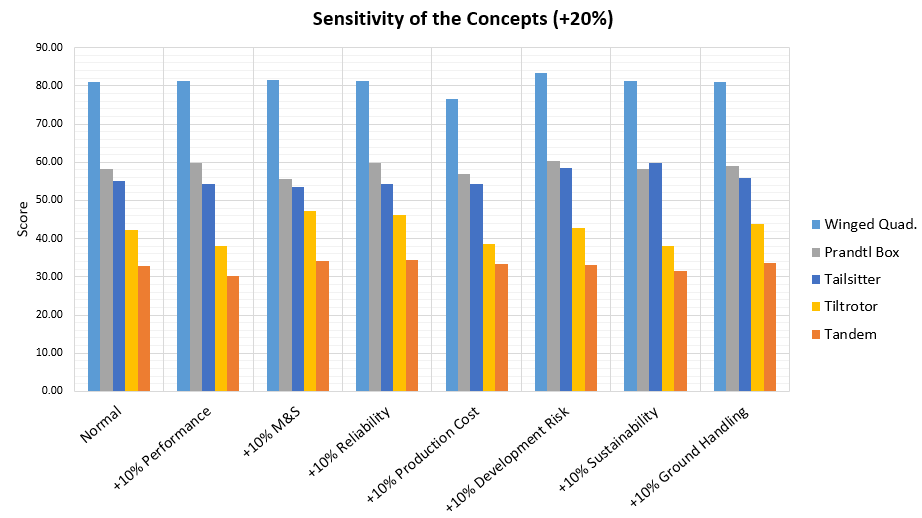
\includegraphics[width=\textwidth]{TradeOff/Figures/sensitivity}
    \caption{Sensitivity Analysis of The Final Trade-Off}
    \label{fig:sensitivityanal}
\end{figure}

The figure shows that even thought the weights of the criteria are changed, The Wing Quadcopter scores highest every time. The gap between the first best and second best does not decrease drastically during the sensitivity analysis, showing that the weighting will not influence the end results. The overall rankings of the concepts also remain unchanged everywhere except when sustainability is weighted 20\% more, this is because The Tailsitter scores 26 higher than The Prandtl Box for that criterion.

Since the Winged Quadcopter greatly outperforms all other concepts throughout the entire sensitivity analysis, it is safe to say that this concept has the greatest potential to satisfy all requirements. Therefore it is sensible to further develop this concept into the preliminary design phase.

